
\documentclass[border=10pt, 12pt]{standalone}
\usepackage[svgnames]{xcolor}
\usepackage{amsmath}
\usepackage{pgfplots}
\pgfplotsset{compat=newest}
\usepackage[sfdefault]{FiraSans}
\usepackage{FiraMono}
\renewcommand*\familydefault{\sfdefault}
\begin{document}
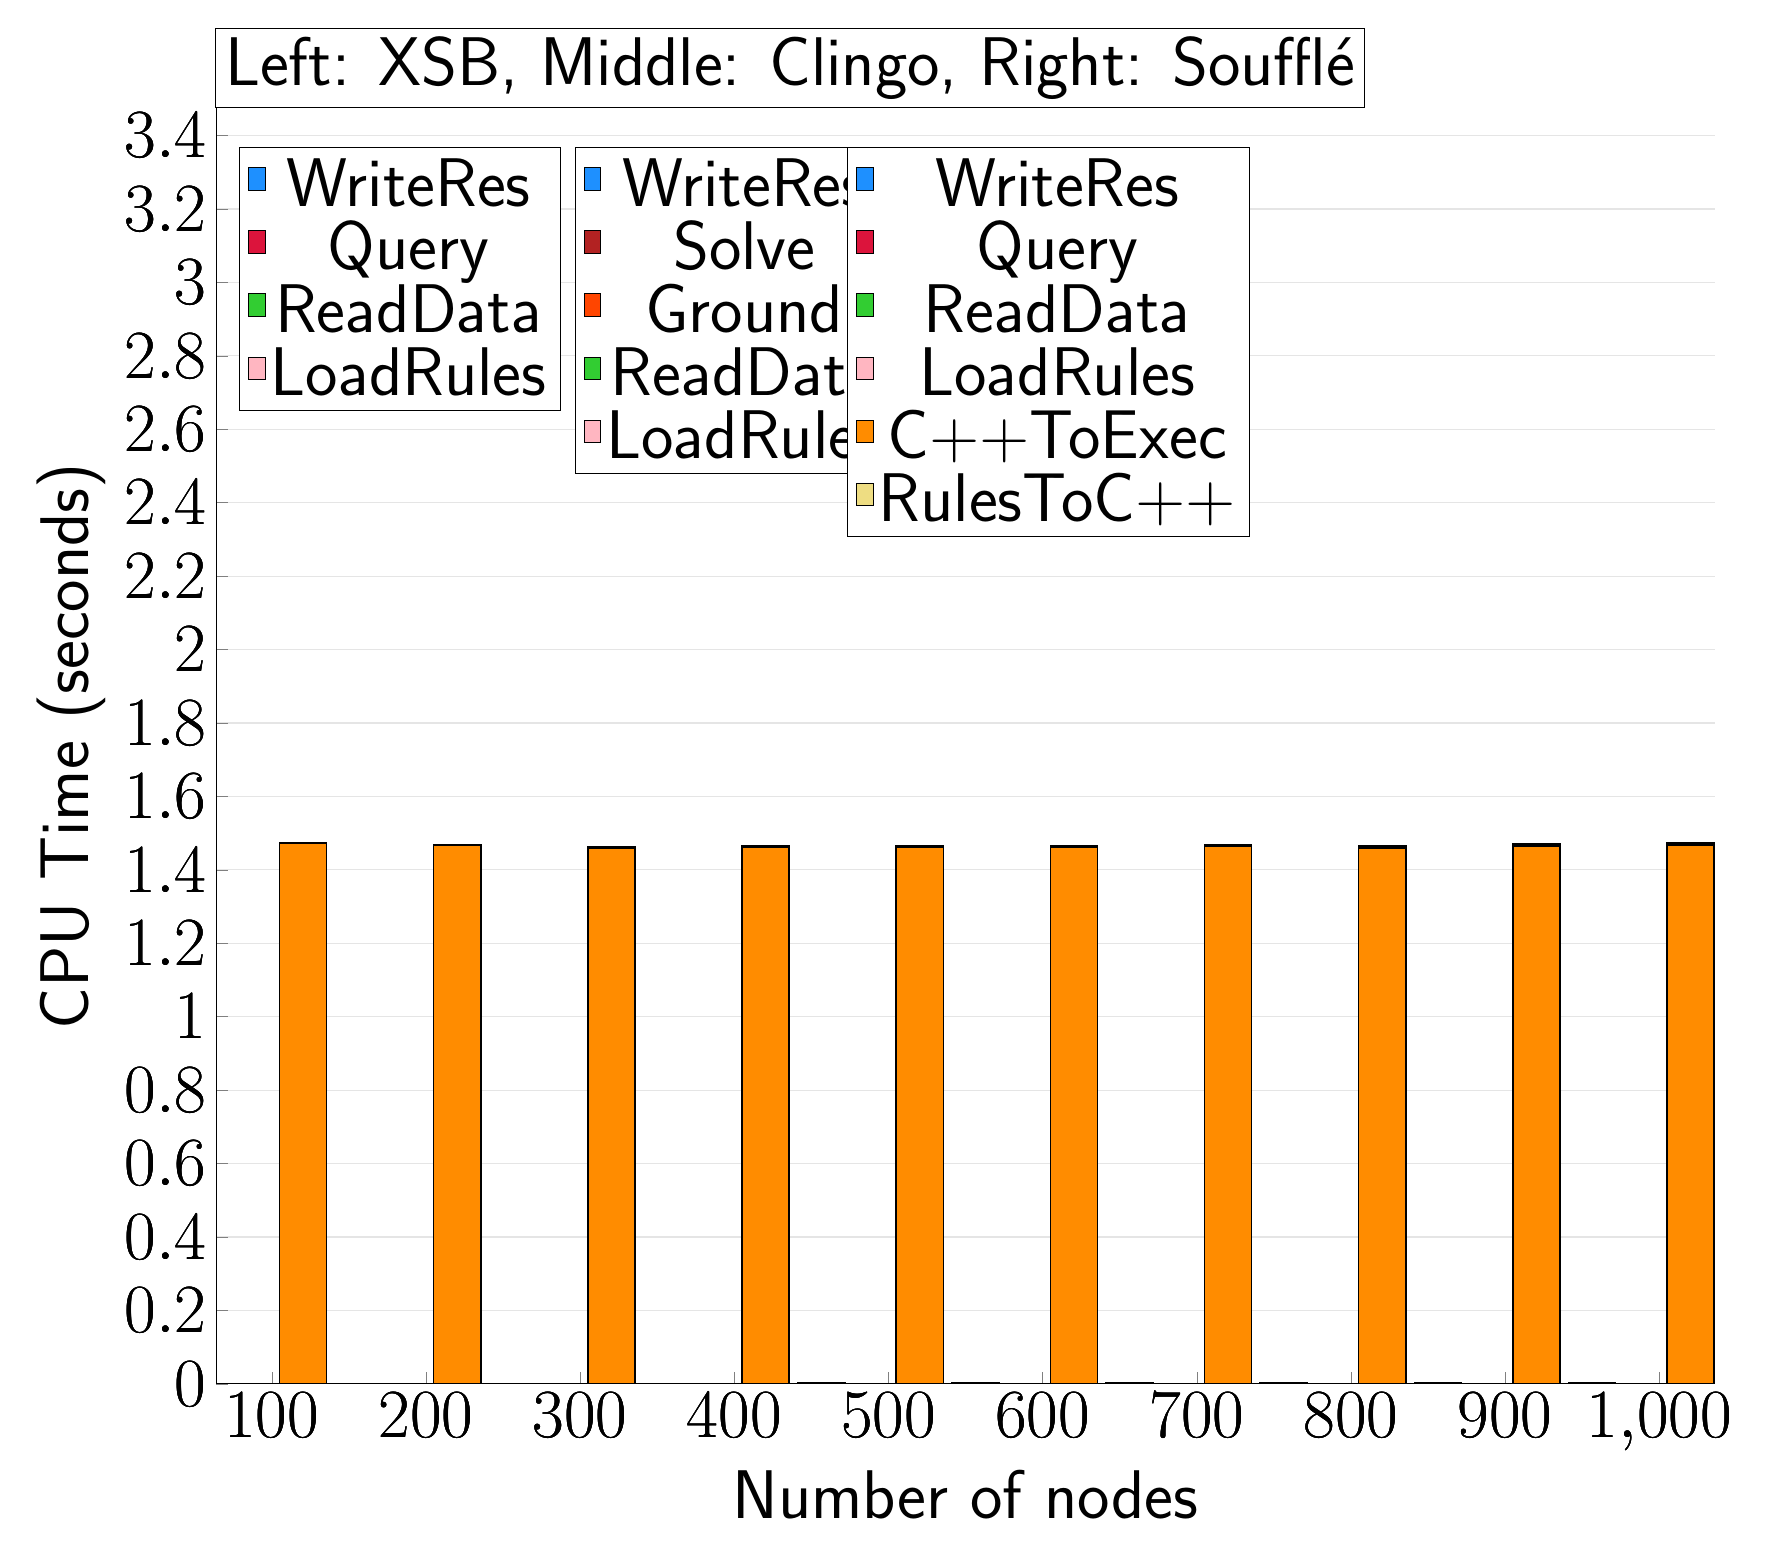
\begin{tikzpicture}
                        \begin{axis}[bar shift=-24.3pt, 
   ybar stacked,
   width=1.7\textwidth,
   bar width=0.6cm,
   ymajorgrids, tick align=inside,
   major grid style={draw=gray!20},
   xtick=data,
   ymin=0, ymax=3.474,
   axis x line*=bottom,
   axis y line*=left,
   enlarge x limits=0.04,
   legend style={
       at={(0.23, 0.97)},
       anchor=north east,
       legend columns=1,
       font=\Huge,
   },
   ylabel={CPU Time (seconds)},
   xlabel={Number of nodes},
   label style={font=\Huge},
   tick label style={font=\Huge},
]
\addlegendimage{fill=DodgerBlue, draw=black, line width=0.2pt}
\addlegendentry{WriteRes}
\addlegendimage{fill=Crimson, draw=black, line width=0.2pt}
\addlegendentry{Query}
\addlegendimage{fill=LimeGreen, draw=black, line width=0.2pt}
\addlegendentry{ReadData}
\addlegendimage{fill=LightPink, draw=black, line width=0.2pt}
\addlegendentry{LoadRules}
\addplot +[fill=LightPink, draw=black, line width=0.55pt] coordinates {
(100, 0.0005621999999999996)
(200, 0.0005507999999999994)
(300, 0.0005586000000000001)
(400, 0.0005627999999999996)
(500, 0.0005546000000000004)
(600, 0.0005585999999999998)
(700, 0.0005496000000000002)
(800, 0.0005576000000000002)
(900, 0.0005494000000000005)
(1000, 0.0005556000000000006)
};
\addplot +[fill=LimeGreen, draw=black, line width=0.55pt] coordinates {
(100, 0.0002003999999999998)
(200, 0.00027759999999999997)
(300, 0.0003552000000000002)
(400, 0.0004206000000000006)
(500, 0.000499)
(600, 0.0005787999999999998)
(700, 0.0006492000000000001)
(800, 0.0007157999999999996)
(900, 0.0008079999999999995)
(1000, 0.0008727999999999993)
};
\addplot +[fill=Crimson, draw=black, line width=0.55pt] coordinates {
(100, 1.7400000000000077e-05)
(200, 2.399999999999972e-05)
(300, 3.559999999999986e-05)
(400, 4.299999999999997e-05)
(500, 5.000000000000074e-05)
(600, 5.959999999999992e-05)
(700, 7.160000000000011e-05)
(800, 8.219999999999964e-05)
(900, 8.979999999999995e-05)
(1000, 9.75999999999998e-05)
};
\addplot +[fill=DodgerBlue, draw=black, line width=0.55pt] coordinates {
(100, 0.00013659999999999953)
(200, 0.0002218000000000005)
(300, 0.0002847999999999999)
(400, 0.00036379999999999984)
(500, 0.0004337999999999995)
(600, 0.0005300000000000004)
(700, 0.0006064)
(800, 0.0007100000000000002)
(900, 0.0007948000000000006)
(1000, 0.0008716000000000008)
};
\end{axis}

\begin{axis}[bar shift=-6.5pt, 
   ybar stacked,
   width=1.7\textwidth,
   bar width=0.6cm,
   ymajorgrids, tick align=inside,
   major grid style={draw=none},
   xtick=data,
   ymin=0, ymax=3.474,
   axis x line*=none,
   axis y line*=none,
   enlarge x limits=0.04,
   legend style={
       at={(0.454, 0.97)},
       anchor=north east,
       legend columns=1,
       font=\Huge,
   },
   label style={font=\Huge},
   tick label style={font=\Huge},
]
\addlegendimage{fill=DodgerBlue, draw=black, line width=0.2pt}
\addlegendentry{WriteRes}
\addlegendimage{fill=FireBrick, draw=black, line width=0.2pt}
\addlegendentry{Solve}
\addlegendimage{fill=OrangeRed, draw=black, line width=0.2pt}
\addlegendentry{Ground}
\addlegendimage{fill=LimeGreen, draw=black, line width=0.2pt}
\addlegendentry{ReadData}
\addlegendimage{fill=LightPink, draw=black, line width=0.2pt}
\addlegendentry{LoadRules}
\addplot +[fill=LightPink, draw=black, line width=0.55pt] coordinates {
(100, 0.0)
(200, 0.0)
(300, 0.0)
(400, 0.0)
(500, 0.0)
(600, 0.0)
(700, 0.0)
(800, 0.0)
(900, 0.0)
(1000, 0.0)
};
\addplot +[fill=LimeGreen, draw=black, line width=0.55pt] coordinates {
(100, 0.0)
(200, 0.0)
(300, 0.0)
(400, 0.0)
(500, 0.0)
(600, 0.0)
(700, 0.0)
(800, 0.0)
(900, 0.0)
(1000, 0.0)
};
\addplot +[fill=OrangeRed, draw=black, line width=0.55pt] coordinates {
(100, 0.0)
(200, 0.0)
(300, 0.0)
(400, 0.0)
(500, 0.0)
(600, 0.0)
(700, 0.0)
(800, 0.0)
(900, 0.0)
(1000, 0.0)
};
\addplot +[fill=FireBrick, draw=black, line width=0.55pt] coordinates {
(100, 0.0)
(200, 0.0)
(300, 0.0)
(400, 0.0)
(500, 0.0)
(600, 0.0)
(700, 0.0)
(800, 0.0)
(900, 0.0)
(1000, 0.0)
};
\addplot +[fill=DodgerBlue, draw=black, line width=0.55pt] coordinates {
(100, 0.0)
(200, 0.0)
(300, 0.0)
(400, 0.0)
(500, 0.0)
(600, 0.0)
(700, 0.0)
(800, 0.0)
(900, 0.0)
(1000, 0.0)
};
\end{axis}

\begin{axis}[bar shift=11.3pt, 
   ybar stacked,
   width=1.7\textwidth,
   bar width=0.6cm,
   ymajorgrids, tick align=inside,
   major grid style={draw=none},
   xtick=data,
   ymin=0, ymax=3.474,
   axis x line*=none,
   axis y line*=none,
   enlarge x limits=0.04,
   legend style={
       at={(0.69, 0.97)},
       anchor=north east,
       legend columns=1,
       font=\Huge,
   },
   label style={font=\Huge},
   tick label style={font=\Huge},
]
\addlegendimage{fill=DodgerBlue, draw=black, line width=0.2pt}
\addlegendentry{WriteRes}
\addlegendimage{fill=Crimson, draw=black, line width=0.2pt}
\addlegendentry{Query}
\addlegendimage{fill=LimeGreen, draw=black, line width=0.2pt}
\addlegendentry{ReadData}
\addlegendimage{fill=LightPink, draw=black, line width=0.2pt}
\addlegendentry{LoadRules}
\addlegendimage{fill=DarkOrange, draw=black, line width=0.2pt}
\addlegendentry{C++ToExec}
\addlegendimage{fill=LightGoldenrod, draw=black, line width=0.2pt}
\addlegendentry{RulesToC++}
\addplot +[fill=LightGoldenrod, draw=black, line width=0.55pt] coordinates {
(100, 0.0)
(200, 0.0)
(300, 0.0)
(400, 0.0)
(500, 0.0)
(600, 0.0)
(700, 0.0)
(800, 0.0)
(900, 0.0)
(1000, 0.0)
};
\addplot +[fill=DarkOrange, draw=black, line width=0.55pt] coordinates {
(100, 1.472)
(200, 1.4659999999999997)
(300, 1.46)
(400, 1.462)
(500, 1.462)
(600, 1.462)
(700, 1.464)
(800, 1.46)
(900, 1.464)
(1000, 1.466)
};
\addplot +[fill=LightPink, draw=black, line width=0.55pt] coordinates {
(100, 0.000148)
(200, 0.00015560000000000001)
(300, 0.0001446)
(400, 0.0001552)
(500, 0.0001496)
(600, 0.0001578)
(700, 0.00015940000000000003)
(800, 0.00016)
(900, 0.00015120000000000002)
(1000, 0.00015599999999999997)
};
\addplot +[fill=LimeGreen, draw=black, line width=0.55pt] coordinates {
(100, 0.0008122000000000001)
(200, 0.0012168)
(300, 0.0015872)
(400, 0.0019682)
(500, 0.0022366)
(600, 0.0027367999999999997)
(700, 0.0028764)
(800, 0.0033772000000000003)
(900, 0.0037278)
(1000, 0.004085)
};
\addplot +[fill=Crimson, draw=black, line width=0.55pt] coordinates {
(100, 0.00017680000000000001)
(200, 0.00035480000000000006)
(300, 0.0005342000000000001)
(400, 0.000691)
(500, 0.0008392)
(600, 0.0009948)
(700, 0.0011196000000000001)
(800, 0.0012502)
(900, 0.0013808000000000002)
(1000, 0.0016764000000000002)
};
\addplot +[fill=DodgerBlue, draw=black, line width=0.55pt] coordinates {
(100, 0.0005013999999999999)
(200, 0.0005054)
(300, 0.0006558)
(400, 0.0007289999999999999)
(500, 0.000735)
(600, 0.0008135999999999999)
(700, 0.0007827999999999999)
(800, 0.0009752000000000001)
(900, 0.0009464)
(1000, 0.0010745999999999998)
};
\end{axis}


\node[anchor=south, draw, fill=white] at (rel axis cs:0.42,1) {\Huge Left: XSB, Middle: Clingo, Right: Soufflé};
\end{tikzpicture}
\end{document}
                    